\scanpage{41}
\mspage{22}
de $\zeta',\zeta_1$ ou de l'une de ces quantités seulement
\[
(75)\qquad\begin{aligned}
\beta'&=\zeta_1\sigma_\infty(\zeta')^{-1}=\deleted{\varepsilon_0(\lambda\zeta_1)}\zeta_1(\sigma_\infty\varepsilon_0)(\lambda\zeta_1)^{-1}\\
&=\lambda^{-1}\cdot\varepsilon_0^{-1}(\zeta')\sigma_\infty(\zeta')^{-1}.
\end{aligned}
\]
de \deleted{la dernière} \inserted{ces} expressions de $\beta'$ on tire
\[
(75')\qquad\begin{aligned}
\sigma_\infty(\beta')&=\sigma_\infty(\zeta_1)\zeta'^{-1}=\sigma_\infty(\zeta_1)\varepsilon_0(\lambda\zeta_1)^{-1}\\
&=\sigma_\infty(\lambda)^{-1}\underbrace{\overbrace{\rho(\zeta')\zeta'^{-1}}^{\alpha'^{-1}}}_{\deleted{\unsure{\alpha'}}}
\end{aligned}
\]
et la troisième expression de $\beta'$ \deleted{donne}

\deleted{$(77)$ Ce dit, l'équation que $(72\,b)$ équivaut à:}
\deleted{\[(77)\qquad\beta'\sigma_\infty(\beta')=1\]}
\deleted{soit, $\sigma_\infty(\beta')$ en posant $\beta_1=\sigma_\infty(\beta')$, pour}
\figure{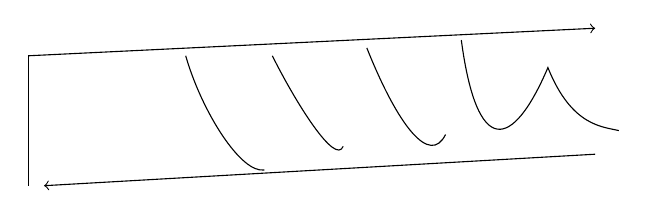
\begin{tikzpicture}[x=1cm,y=1cm]\draw[->] (0,1)--(7.2,1.35);\draw (0,1)--(0,-.65);\draw[->] (7.2,-.25)--(.2,-.65);\draw (2,1)..controls (2.2,.3) and (2.7,-.5)..(3,-.45);\draw (3.1,1)..controls (3.4,.4) and (3.9,-.4)..(4,-.15);\draw (4.3,1.1)..controls (4.7,.1) and (5.1,-.4)..(5.3,0);\draw (5.5,1.2)..controls (5.7,-.3) and (6.15,-.2)..(6.6,.85)..controls (6.9,.1) and (7.3,.1)..(7.5,.05);\end{tikzpicture}}
s'écrit aussi
\[
(77)\qquad\sigma_\infty(\beta')^{-1}=\alpha'\sigma_\infty(\lambda).
\]
Ceci posé, l'équation $(72\,b)$ équivaut à
\[
(78)\qquad\beta'\sigma_\infty(\beta')=1\qquad\text{ou encore}\quad\sigma_\infty(\beta')^{-1}=\beta'
\]
ce qui est invariant par la substitution $\beta'\mapsto\sigma_\infty(\beta')$ \unsure{ou|\deleted{dans}} $\beta'\mapsto\beta'^{-1}$, donc posant
\inserted{(sans supposer vérifiée $(*)$)}
\[
\beta_1=\sigma_\infty(\beta')^{-1}=\alpha'\sigma_\infty(\lambda)
\]
l'équation (78) équivaut à l'équation
\[
(**)\qquad\beta_1\sigma_\infty(\beta_1)=1
\]
et implique que $\beta_1=\sigma_\infty(\beta_1)^{-1}$ donc $\beta_1=\beta'$.

En résumé, on peut tout de suite poser
\[
(79)\qquad\beta'=\alpha'\sigma_\infty(\lambda)\qquad\text{où}\quad\alpha'=\zeta'\rho(\zeta')^{-1}
\]
et la relation à imposer à $(\lambda,\zeta')$ est, au choix,
\margin{40}
